\documentclass{article}
\usepackage[utf8]{inputenc}
\usepackage{mathtext}
\usepackage{amsmath}
\usepackage[colorlinks=true, linkcolor=orange]{hyperref}
\usepackage[T1]{fontenc}
\usepackage[utf8]{inputenc}
\usepackage[english, bulgarian, russian]{babel}
\usepackage{tikz}
\usepackage{pgfplots}
\usepackage{indentfirst}
\usepackage[export]{adjustbox}
\usepackage{lipsum} % sample text
\usepackage{floatflt}
\usepackage{multirow}
\usepackage{geometry}


\geometry{verbose,a4paper,tmargin=2cm,bmargin=2cm,lmargin=1.5cm,rmargin=1.5cm}
\setlength{\parindent}{0.65cm}
\setlength{\parskip}{0.15cm}

\usepackage{wrapfig}
\usepackage{array,graphicx,caption}


%Матеша
\usepackage{amsmath,amsfonts,amssymb,amsthm,mathtools,  mathrsfs, wasysym} % AMS
\usepackage{icomma} % "Умная" запятая

%\mathtoolsset{showonlyrefs=true} % Показывать номера только у тех формул, на которые есть \eqref{} в тексте.

%% Шрифты
\usepackage{euscript}	 % Шрифт Евклид
\usepackage{mathrsfs} % Красивый матшрифт

%% Свои команды
\DeclareMathOperator{\sgn}{\mathop{sgn}}

%% Перенос знаков в формулах (по Львовскому)
\newcommand*{\hm}[1]{#1\nobreak\discretionary{}
	{\hbox{$\mathsurround=0pt #1$}}{}}


% Рисунки
\usepackage{subcaption,floatrow,graphicx,calc}
\usepackage{wrapfig}


% Создаёем новый разделитель
\DeclareFloatSeparators{mysep}{\hspace{1cm}}

\DeclareUnicodeCharacter{0306}{~}


\begin{document}
\def\figurename{Рисунок}
\begin{titlepage}
\begin{center}
    {\large МОСКОВСКИЙ ФИЗИКО-ТЕХНИЧЕСКИЙ ИНСТИТУТ (НАЦИОНАЛЬНЫЙ ИССЛЕДОВАТЕЛЬСКИЙ УНИВЕРСИТЕТ)}
\end{center}
\begin{center}
    {\largeФизтех-школа биологической и медицинской физики}
\end{center}

\vspace{1cm}
{\huge
\begin{center}
    {\bf Лабораторная работа по физическим методам исследования}\\
    \vspace{0.5cm}
    Спектроскопия электронного парамагнитного резонанса  
\end{center}
}

\vspace{4cm}
\begin{flushright}
{\LARGE Выполнили студенты группы Б06-103:\\Попеску Полина \\ Фитэль Алена}

\end{flushright}
\vspace{9cm}
\begin{center}
    Долгопрудный, 2024 г.
\end{center}
\end{titlepage}



\newpage

\setcounter{page}{2}

	\textbf{Цели работы:} исследование
сверхтонкой структуры спектров электронного парамагнитного резонанса (ЭПР), измерение скорости спин-спинового обмена в растворах и кристаллах, исследование влияния амплитуды
высокочастотной модуляции и уровня диэлектрических потерь на
вид спектров ЭПР.


\section{Теоретическое введение}
Электронный парамагнитный резонанс (ЭПР) как метод исследования
был разработан Е. К. Завойским с сотрудниками С. А. Альтшулером и
Б. М. Козыревым в 1944 г. в Казани. Созданию метода предшествовали
открытие спина электрона, открытие эффекта Зеемана, а также длительная
работа, направленная на поиск возможности применения полей
радиочастотного диапазона для исследования веществ.
Метод электронного парамагнитного резонанса применяется для
исследования парамагнитных центров и их окружения в веществе.
Методом ЭПР можно определять концентрацию и идентифицировать
парамагнитные частицы в любом агрегатном состоянии. Он позволяет
детектировать свободные радикалы в количестве до $10^{-10}$---$10^{-13}$ М.
\subsection{Явление электронного парамагнитного резонанса}

Избирательное поглощение энергии излучения системой парамагнитных  частиц во внешнем магнитном поле получило название электронного парамагнитного резонанса.

В квантовой теории проекция орбитального момента импульса на заданную ось (z) и его квадрат могут принимать лишь дискретные значения:

\begin{equation}
\begin{aligned}
l_{z}=m_{l}\hbar \\
l^{2}=l(l+1)\hbar^{2} \\
m_l = -l, \dots, l
\end{aligned}
\end{equation}

Где $m_l$ и $l$ --- магнитное и орбитальное квантовые числа, $\hbar$ = 1.05$\cdot$10\textsuperscript{-27} эрг$\cdot$с – постоянная Планка. Орбитальному движению электрона соответствует магнитный момент, проекцию которого можно выразить через гиромагнитное отношение:

\begin{equation}
\mu _{z}= \gamma l_{z}=-\frac{e}{2mc}\hbar m_{l}
\end{equation}

Удобно ввести магнетон Бора $\beta =\frac{e}{2mc}\hbar = 9.274\cdot10^{-21}$ эрг/Гс и безразмерную величину гиромагнитного отношения --- g--фактор. Проекцию магнитного момента принято писать в виде:

\begin{equation}
\mu _{z}=-g_{l} \beta m_{l}
\end{equation}

Проекции спина и спинового магнитного момента:

\begin{equation}
\begin{aligned}
s_{z}=m_{s}\hbar            \\
m_{s}=-s, \dots ,s          \\
\mu _{z}=-g_{s} \beta m_{s}
\end{aligned}
\end{equation}


\begin{figure}[h!]
%	\vspace{-30pt}
	\begin{center}
		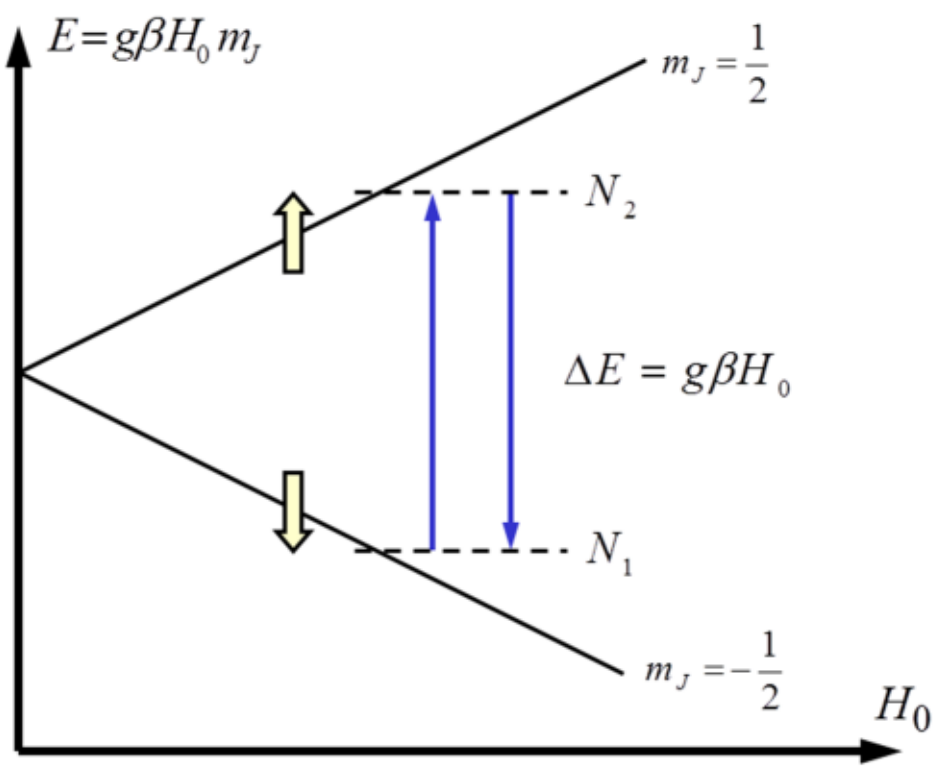
\includegraphics[width=0.45\textwidth]{pic1.png}
	\end{center}
%	\vspace{-20pt}
	\caption{Энергетические уровни электрона во внешнем магнитном поле \textbf{H}\textsubscript{0}}
	\label{pic1}
\end{figure}

где s – спиновое квантовое число электрона, равное s=1/2. Чисто спиновый g-фактор свободного электрона g\textsubscript{s}=2. Если атомная частица содержит несколько электронов, то их орбитальные и спиновые моменты складываются, магнитные свойства частицы будут определяться значениями квантовых чисел L и S. Полный механический момент частицы J=L+S

Спин-орбитальное взаимодействие является возмущением, смешивающим волновые функции основного состояния с волновыми функциями возбужденных орбитальных состояний радикала, что приводит к отклонению величин g-факторов радикалов от чисто спинового значения g\textsubscript{s}:

\begin{equation}
g=g_{s} \left( 1-\frac{a \lambda _{SL}}{ \Delta E} \right)
\end{equation}

где $\Delta E$ – расщепление между основным и ближайшим по энергии орбитальным состоянием, участвующим в орбитальном движении; $а$ – множитель, который зависит от природы парамагнитного центра и ориентации его по отношению к внешнему магнитному полю.

Для определенности далее будем рассматривать частицы с чисто спиновым магнитным моментом (J = S, L = 0). При включении внешнего магнитного поля \textbf{H}\textsubscript{0} появляется выделенное направление, так что энергия магнитного диполя:

\begin{equation}
E = - (\mu , H_{0}) = g \beta H_{0}m_{J}
\end{equation}

Согласно квантовомеханическим правилам отбора, $ \Delta m_{J}$ = $ \pm $ 1, что приводит к возможности переходов с энергией:

\begin{equation}
h\nu = \Delta E = g \beta H_{0}
\end{equation}

\subsection{Сверхтонкая структура линий ЭПР спектра}

В том случае, если ядро атома также обладает магнитным моментом, структура линий ЭПР спектра становится более сложной. При достаточно больших внешних полях произойдет «разрыв» связи ядра и электронной оболочки, магнитные моменты ядра и электронной оболочки будут ориентироваться во внешнем магнитном поле независимо друг от друга. На электрон будет действовать локальное магнитное поле $H_0 + \Delta H$, где $ \Delta H$ – дополнительное магнитное поле, созданное ядром. Такое взаимодействие магнитных моментов электрона и ядра приводит к изменению условия резонанса и носит название сверхтонкого взаимодействия (СТВ).

\begin{figure}[h!]
	\begin{center}
		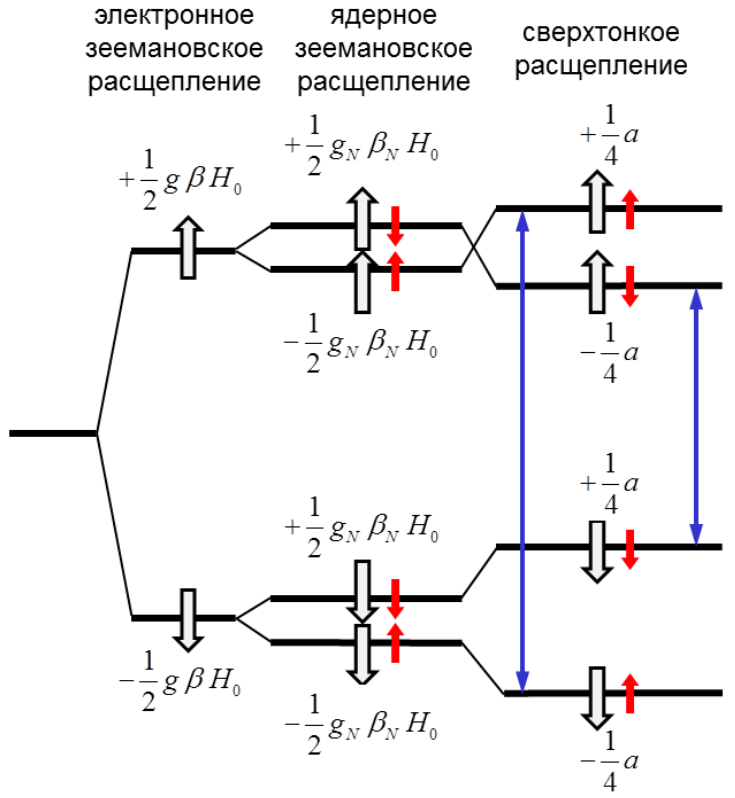
\includegraphics[width=0.6\textwidth]{pic2.png}
	\end{center}
	\caption{Образование тонкой структуры спектра ЭПР для атома водорода}
	\label{pic2}
\end{figure}

Ориентация магнитных моментов ядер во внешнем магнитном поле так же подчиняется квантово-механическим правилам квантования, как и ориентация магнитных моментов электронов. Важно отметить также, что времена пребывания ядер в состояниях с определенной ориентацией магнитного момента (времена спин-решеточной релаксации для ядер) относительно велики и лежат в диапазоне 10\textsuperscript{-3} --- 1 с. Следовательно, рассматривая переходы между электронными зеемановскими уровнями, магнитные моменты ядер стоит считать фиксированными. Тогда электроны различных атомов будут находиться в магнитных полях, создаваемых ядрами, имеющих $2I + 1$ различных значений. Условие резонанса при плавном изменении внешнего магнитного поля будет выполняться для электронов $2I + 1$ раз, т.е. произойдет расщепление линии поглощения. Расстояние между линиями сверхтонкой структуры называют константой сверхтонкого взаимодействия $ \alpha $.

Характерным признаком для расщепления линий в спектре ЭПР под влиянием парамагнитных ядер одиночных атомов является равная интенсивность всех линий.

Для многоатомного радикала c суммарным спином $S = 1/2$, локальное магнитное поле будет определяться суммарным действием нескольких близлежащих магнитных ядер. Общую энергию системы в этом случае можно записать:

\begin{equation}
E = g \beta H_{0}m_{s}+ \sum g_{i} \beta _{яд}H_{0}m_{i} + \sum g \beta a_{i}m_{s}m_{i}
\end{equation}

Правила отбора для переходов, возбуждаемых при ЭПР:

\begin{equation}
\begin{aligned}
\Delta m_{S}= \pm 1 \\
\Delta m_{i} = 0
\end{aligned}
\end{equation}

\subsection{Скорость поглощения энергии при ЭПР}

Одним из важных применений метода ЭПР является определение числа парамагнитных частиц в образце по величине поглощаемой при резонансе мощности электромагнитной энергии.

Заселённости уровней в отсутствие поглощения энергии будут определяться константами скорости спонтанных переходов $K_{1}$ и $K_{2}$:

\begin{equation}
\frac{N_{2}}{N_{1}}=\frac{K_{1}}{K_{2}}=\exp\left( -\frac{ \Delta E}{kT} \right)
\end{equation}

$N_1$ и $N_2$ – число частиц на каждом из подуровней. При T$ \sim $ 300$ ^{\circ} $ C и Н$ \sim $ 3000 Э будет выполняться $ \Delta E/kT \ll 1 ( \Delta E/kT \sim 10^{-3})$. Тогда, при разложении в ряд, получим: $N_2/N_1 = 1 - \Delta E/kT $.

При резонансном поглощении энергии возникают вынужденные (индуцированные) переходы, характеризующиеся вероятностью переходов в единицу времени  $K_{ind}=kH_{1}^{2}$, пропорциональной квадрату напряженности переменного магнитного поля $H_1$. Энергия, поглощаемая в единицу времени, будет определяться соотношением:

\begin{equation}
W= \Delta EK_{ind} \left( N_{1}-N_{2} \right) =\frac{ \Delta E^{2}}{kT}\frac{N}{2}\frac{K_{ind}}{1+\frac{K_{ind}}{K_{1}}}
\end{equation}

Из этого выражения следует, что скорость поглощения энергии пропорциональна числу парамагнитных частиц N. Именно этот факт позволяет оценивать число парамагнитных частиц в образце путем измерения мощности поглощения при электронном парамагнитном резонансе.

\subsection{Уширение линий и релаксационные процессы}

Ширина линии поглощения и ширина уровня энергии связаны со временем жизни частицы на определенном уровне энергии $\tau$  соотношением неопределенностей:

\begin{equation}
\begin{aligned}
\delta\omega\tau \sim 1 \\
\delta E\tau \sim \hbar
\end{aligned}
\end{equation}

Время жизни $\tau$  определяется релаксационными процессами, происходящими при взаимодействии спинов друг с другом и с другими степенями свободы системы (с так называемой решеткой, вне зависимости от наличия реальной кристаллической решетки). \par

Существуют два типа релаксационных процессов. Во-первых, это продольная релаксация, то есть релаксация продольной намагниченности образца к ее равновесному значению вдоль внешнего постоянного магнитного поля: $M_z \rightarrow M_0 $. Энергия из спиновой системы при этом передается в решетку. Поэтому такую релаксацию называют также спин-решеточной. Скорость релаксации характеризуют временем продольной релаксации $T_1$, за которое продольная компонента намагниченности спиновой системы уменьшается в е раз.

Второй тип релаксационных процессов – поперечная релаксация. Она приводит к обнулению поперечных компонент вектора намагниченности образца $ M_x, M_y \rightarrow 0$. В отличие от продольной, в ходе поперечной релаксации энергия спиновой системы не изменяется. В процессе поперечной релаксации происходит разориентация вкладов в поперечную намагниченность от магнитных моментов, находящихся в различных локальных магнитных полях. Разориентация может быть обусловлена как различием частот прецессии векторов намагниченности в неоднородном магнитном поле, так и спинспиновой релаксацией, при которой взаимодействие двух частиц приводит к изменению спиновых состояний каждой из них (например, обмен спинами). Характерное время, необходимое для данного типа релаксации вектора намагниченности, называют временем поперечной релаксации $T_2$.

Поскольку взаимодействие спинов с решеткой также приводит к расфазировке прецессии магнитных моментов, оно также вносит вклад в процесс поперечной релаксации, наравне со спин-спиновой:

\begin{equation}
\frac{1}{T_{2}}=\frac{1}{T_{1}}+\frac{1}{ \tau_{ss}}>\frac{1}{T_{1}}
\end{equation}

Таким образом, время $T_2$ меньше $T_1$. Оно ограничивает время жизни спинового состояния и определяет ширину резонансных линий $\delta  \omega$. Выражая ширину линии в единицах магнитного поля, получим следующее соотношение:

\begin{equation}
\delta H \left[ \text{Э} \right] =\frac{ \delta  \omega }{ \gamma }=\frac{\hslash}{g \beta T_{2}} \approx 5\cdot10^{-8}\frac{1}{T_{2} \left[ c \right] }
\end{equation}

Уширение линий за счет спин-спинового взаимодействия может быть уменьшено путем уменьшения концентрации парамагнитных частиц.

Рассмотрим несколько подробнее процесс спин-спиновой релаксации при спиновом обмене. При столкновении двух парамагнитных частиц в растворе между ними возникает обменное взаимодействие (если электронные оболочки неспаренных электронов перекрываются), при котором частица 1 приобретает спиновое состояние частицы 2, а частица 2 приобретает спиновое состояние частицы 1. Скорость спинового обмена пропорциональна частоте двойных соударений парамагнитных частиц, т.е. пропорциональна концентрации C [М] парамагнитных частиц в растворе:

\begin{equation}
\frac{1}{ \tau_{e}}=K_{e}C
\end{equation}
где $K_e$– константа спинового обмена.

В результате обмена спин электрона может оказаться в другом магнитном окружении.

Пусть $ \Delta  \omega $  - разница резонансных частот при различном магнитном окружении в отсутствии спинового обмена. В случае медленного обмена, при $1/ \tau_e \ll \Delta \omega $ , расщепление линии на отдельные компоненты сохранится, но при этом сократится время пребывания электрона в состоянии с тем или иным магнитным окружением. В соответствии с соотношением неопределенности это приведет к уширению каждой из компонент расщепленной линии:

\begin{equation}\label{spin}
\delta H_{e}=\cfrac{1}{\gamma \tau_e} = K_e C \cfrac{1}{\gamma}
\end{equation}

\subsection{Форма линий в спектре ЭПР}
Мощность поглощаемой образцом электромагнитной энергии пропорциональна интенсивности сигнала, т.е. площади под кривой поглощения S. Численно значение площади под кривой линии поглощения можно получить либо дважды продифференцировав полученный с ЭПР-спектрометра сигнал, либо по приближенной формуле: 

\begin{equation}\label{s}
Y_{max}^{'} \left(  \Delta H_{max} \right) ^{2}\sim S,
\end{equation}
где $2Y_{max}^{'}$ - амплитуда между точками максимального наклона, $ \Delta $ $H_{max}$ – расстояние между экстремумами первой производной сигнала. Соотношение между шириной линии спектра на полувысоте $ \delta H $ и $ \Delta H_{max}$ зависит от формы линии спектра.

\begin{equation}
y=\frac{a}{1+bx^{2}} - \text{Лоренцев контур}; \Delta H_{max} = \frac{2}{\sqrt{3}}\delta H
\end{equation}
 

\begin{equation}
y=ae^{-bx^{2}} - \text{Гауссов контур}; \Delta H_{max} = \sqrt{\frac{2}{\ln 2}}\delta H
\end{equation}

\begin{figure}[h!]
	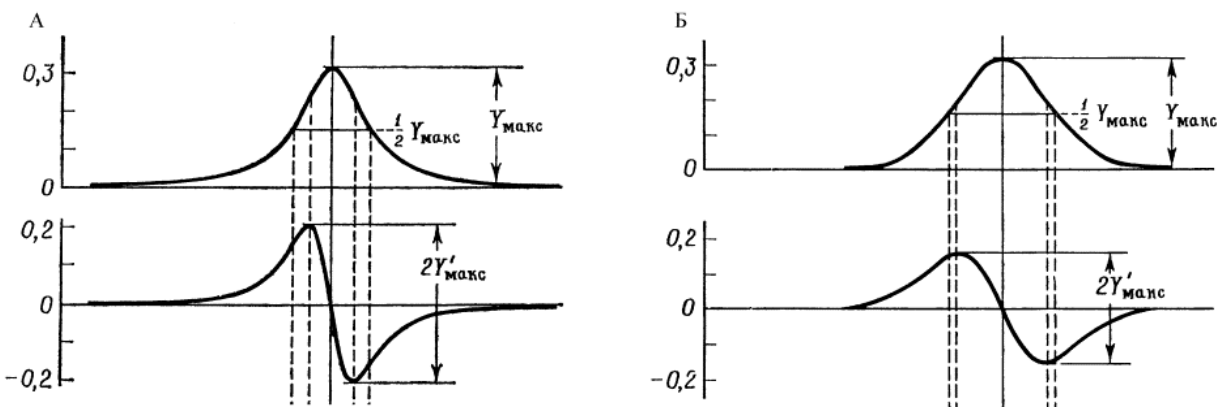
\includegraphics[scale = 0.5]{pic4.png}
	\caption{Кривые поглощения и их первые производные в форме Лоренца (А) и
		Гаусса (Б)}
	\label{cont}
\end{figure}

\section{Ход работы и обработка результатов}

\subsection{Исследование влияния амплитуды высокочастотной модуляции на вид спектров ЭПР}
\begin{enumerate}
    \item В ходе работы были зарегистрированы спектры ЭПР ДФПГ при разных амплитудах модуляции магнитного поля, определяемых силой тока в модуляционных катушках в диапазоне $0.05 - 1 А$. На \hyperref[1_all]{Рисунке \ref*{1_all}} видно, что с увеличением амплитуды модуляции амплитуда сигнала и расстояние между экстремумами увеличивается. 

\begin{figure}[h!]
        \centering
        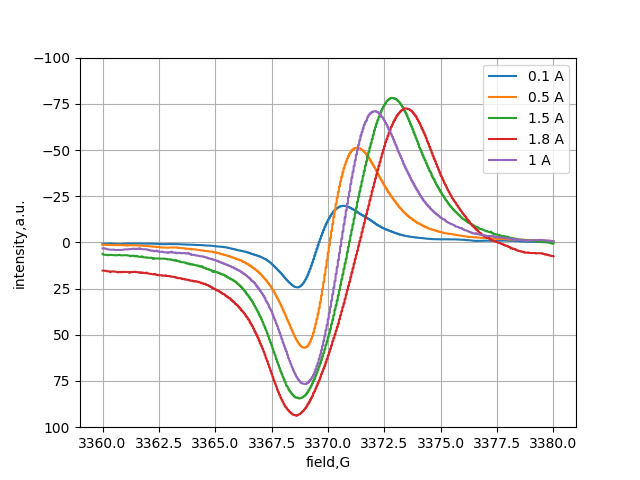
\includegraphics[scale = 0.9]{1/1_all.png}
        \caption{Спектры ЭПР ДФПГ при разных токах модуляции}
        \label{1_all}
    \end{figure}
    \item Интегральная интенсивность ЭПР спектра может быть описана лоренцевым контуром $y=\frac{a}{1+b(x-x_0)^2}$. Полуширина контура на полувысоте может быть получена следующим образом:
    
\begin{equation*}
    \frac{y(x_0+\delta x)}{y(x_0)} = \frac{a/(1+b(\delta x-x_0)^2}{a} = \frac{1}{1+b(\delta x-x_0)^2} = \frac{1}{2}
\end{equation*}
\begin{equation*}
    \delta x = \frac{1}{\sqrt{b}}, \sigma \delta x = \frac{1}{2b^{3/2}}\sigma b
\end{equation*}
   
    \item Используя эти формулы проведем интегрирование экспериментальных спектров и фитирование полученных кривых, рассчитаем полуширину линии поглощения $\delta H$ для каждой величины тока модуляции и построим их зависмость от величины тока модуляции(\hyperref[1__]{Рисунок \ref*{1__}} (Приложение), \hyperref[table1]{Таблица \ref*{table1}}, \hyperref[1_final]{Рисунок \ref*{1_final}}).


\begin{table}[h!]
\centering
\begin{tabular}{|c|c|c|}
\hline
I, mA & $\delta H$ & $\sigma \delta H$ \\ \hline
0.1   & 1.623      & 0.014             \\ \hline
0.5   & 1.708      & 0.012             \\ \hline
1.0   & 1.99       & 0.09              \\ \hline
1.5   & 2.45       & 0.11              \\ \hline
1.8   & 2.23       & 0.4               \\ \hline
\end{tabular}
\caption{Полуширина интегральных кривых ЭПР спректра на полувысоте для ДФПГ при разных амплитудах модуляции МП}
\label{table1}
\end{table}

\begin{figure}[h!]
        \centering
        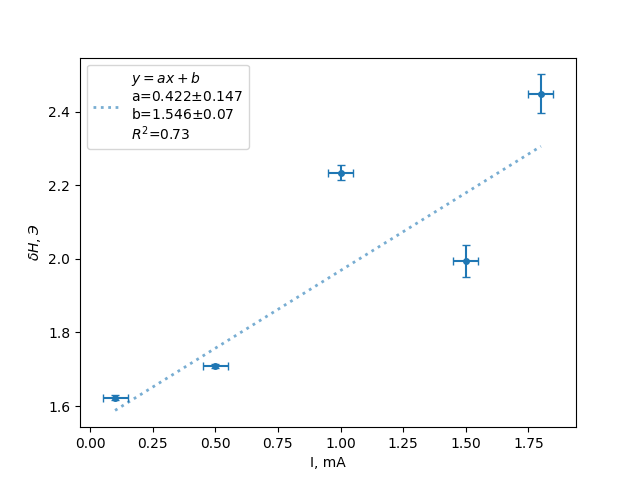
\includegraphics[scale = 0.8]{1/1_final.png}
        \caption{Зависимость полуширины линий поглощения $\delta H$ от величины тока модуляции для спектра ЭПР ДФПГ}
        \label{1_final}
    \end{figure}


\item Видно, что зависимость линейная с хорошей точностью. Минимальная достижимая амиплитуда модуляции (при I=0) $\delta H =  1,55 \pm 0,07\text{Э}$.

\end{enumerate}

\subsection{Исследование скорости спинового обмена в растворах и кристаллах}


\subsubsection{Исследование в растворaх}
 \begin{itemize}
 \item Были зарегистрированы спектры ЭПР при разных концентрациях соли $Mn^{2+}$. На \hyperref[2_all]{Рисунке \ref*{2_all}}, как с увеличением концентрации уменьшается амплитуда сигнала, но положения экстремумов остаётся практически теми же.

\item В \hyperref[table2]{Таблице \ref*{table2}} приведена информация о полуширинах линии поглощения при различных концентрациях раствора (\hyperref[2__]{Рисунок \ref*{2__}} (Приложение)). На \hyperref[2_final_lin]{Рисунке \ref*{2_final_lin}} приведён график зависимости полуширины линии поглощения от концентрации образца. 


\begin{figure}[h!]
        \centering
        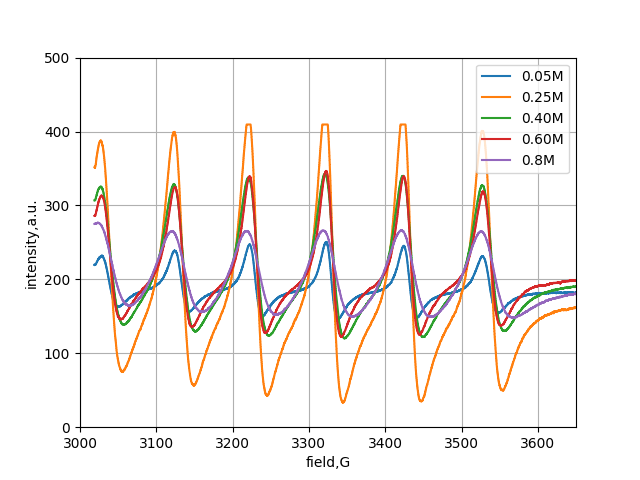
\includegraphics[scale = 0.8]{2.1/2_all.png}
        \caption{Спектры ЭПР раствора $MnSO_4$ при разных концентрациях}
        \label{2_all}
    \end{figure}

\begin{table}[h!]
\centering
\begin{tabular}{|c|c|c|}
\hline
c, мМ & $\delta H$ & $\sigma \delta H$ \\ \hline
0.05  & 10.0       & 0.3               \\ \hline
0.25  & 14.6       & 0.2               \\ \hline
0.40  & 15.6       & 0.2               \\ \hline
0.60  & 13.5       & 0.2               \\ \hline
0.80  & 18.4       & 0.3               \\ \hline
\end{tabular}
\caption{Полуширина интегральных кривых ЭПР спректра на полувысоте для растворов $Mn^(+2)$ при разных концентрациях}
\label{table2}
\end{table}


\begin{figure}[h!]
        \centering
        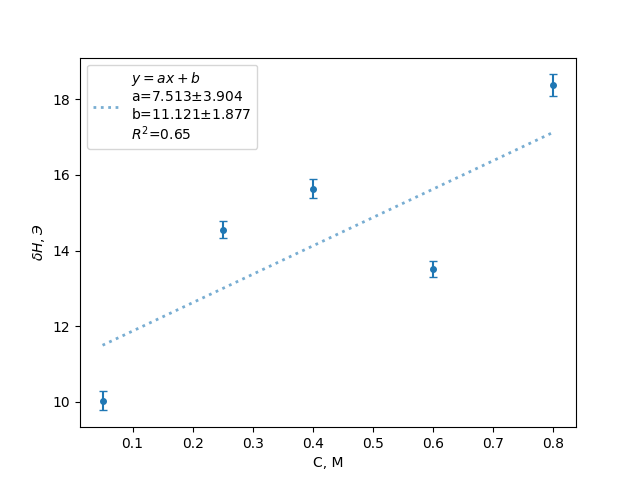
\includegraphics[scale = 0.8]{2.1/2_final_lin.png}
        \caption{Зависимость полуширины линий поглощения спектра ЭПР $\delta H$ от величины концентрации растворов $MnSO_4$}
        \label{2_final_lin}
    \end{figure}




\item Согласно теоретическому введению, константа спинового обмена ($\gamma =   17.6 \cdot 10^6$ 1/(Э·c)):
\begin{equation*}
    \delta H = K_e \cdot C \cdot \frac{1}{\gamma} \Rightarrow K_e = \gamma \cdot a, \sigma K_e = \gamma \sigma a
\end{equation*}

\begin{equation*}
    K_e = (1.3 \pm 0.7)\cdot 10^8 M^{-1}c^{-1}
\end{equation*}

\item Частота столновений парамагнитных частиц в растворе:
\begin{equation*}
    \frac{1}{\tau_e} = K_e\cdot C
\end{equation*}
Оценка для C=0.6M:
\begin{equation*}
    \frac{1}{\tau_e} = (0.08 \pm 0.04) \text{ГГц}
\end{equation*}

\item  Также была получена зависимость поглощения энергии СВЧ-поля от концентрации раствора (\hyperref[2_final_exp]{Рисунок \ref*{2_final_exp}}).


\begin{figure}[h!]
        \centering
        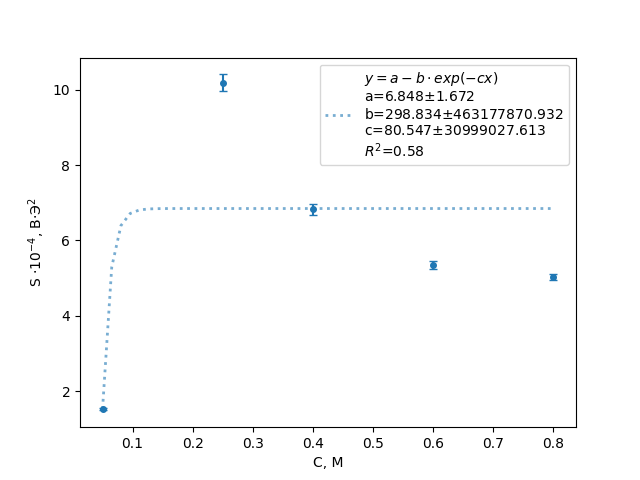
\includegraphics[scale = 0.7]{2.1/2_final_exp.png}
        \caption{Зависимость поглощения СВЧ-поля от концентрации раствора $MnSO_4$}
        \label{2_final_exp}
    \end{figure}

\end{itemize}

\newpage
\subsubsection{Исследование в кристаллах}
Был снят спектр порошка соли $Mn^{2+}$  (\hyperref[2_sold]{Рисунок \ref*{2_sold}}).
Как видно из графика, для $Mn^{2+}$ в кристаллическом виде наблюдается быстрый спиновый обмен:  в спектре наблюдается только одна линия резонанса (т.е. электронный спин, фактически, находится в 
усредненном магнитном поле).

\begin{figure}[h!]
        \centering
        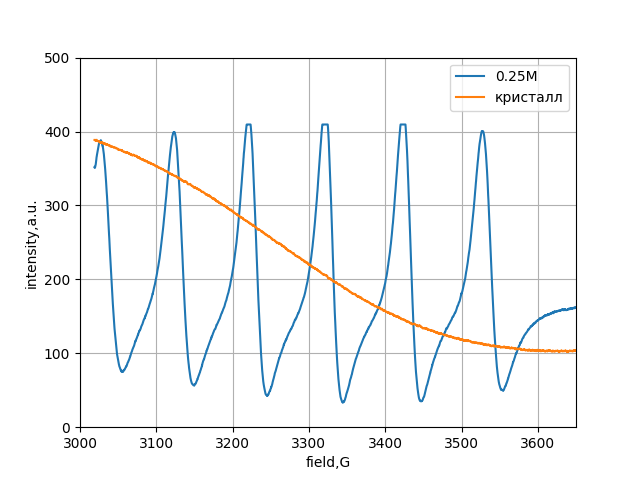
\includegraphics[scale = 0.7]{2_sold.png}
        \caption{Спектр ЭПР соли $Mn^{2+}$ в кристаллическом виде и в растворе при концентрации $c = 0.25 M$}
        \label{2_sold}
    \end{figure}

\subsection{Исследование сверхтонкой структуры спектров ЭПР}

\subsubsection{Определение константы сверхтонкого взаимодействия по спектру $Mn^{2+}$}
На ЭПР спектре $Mn^{2+}$ (\hyperref[2_final_exp]{Рисунок \ref*{2_final_exp}}) наблюдалось 6 эквидистатных пиков равной интенсивности. Это линии сверхтонкой структуры, обусловленные взаимодействием магнитных моментов электрона и ядра. Число линий спектра - это число проекций спина на направление МП. В данном случае $6=2\cdot I + 1$, т.е. спин ядра Mn равен $I=\frac{5}{2}$. Одинаковая интенсивность пиков указывает на то, что заселенности уровней практически одинаковы: т.к. разница энергии ядер на уровнях с различными проекциями спина много меньше тепловой энергии,то  равновесные заселенности уровней, соответствующие различным
ориентациям ядер, одинаковы.\\
С учетом эквидистантности линий сверхтонкого расщепления, оценка постоянной сверхтонкого расщепления производилась по расстоянию между пиками поглощения (интерполяция производной). Результат расчетов:

\begin{equation*}   
    a=(100.1 \pm 0.9)\text{ Э}
\end{equation*}

\subsubsection{Спектр $Ca(OH)_2$}

В спектре ЭПР порошка $Ca(OH)_2$ (\hyperref[3]{Рисунок \ref*{3}}) обнаружено  6 линий поглощения. Значит,  в веществе
находится парамагнитный центр со спином ядра $I=5/2$. Так как вещество состоит из молекул  $Ca(OH)_2$, то данный спин соответствует изотопу $O^{17}$( доля $O^{17}$ в природе: $0.038\%$).

\begin{figure}[h!]
        \centering
        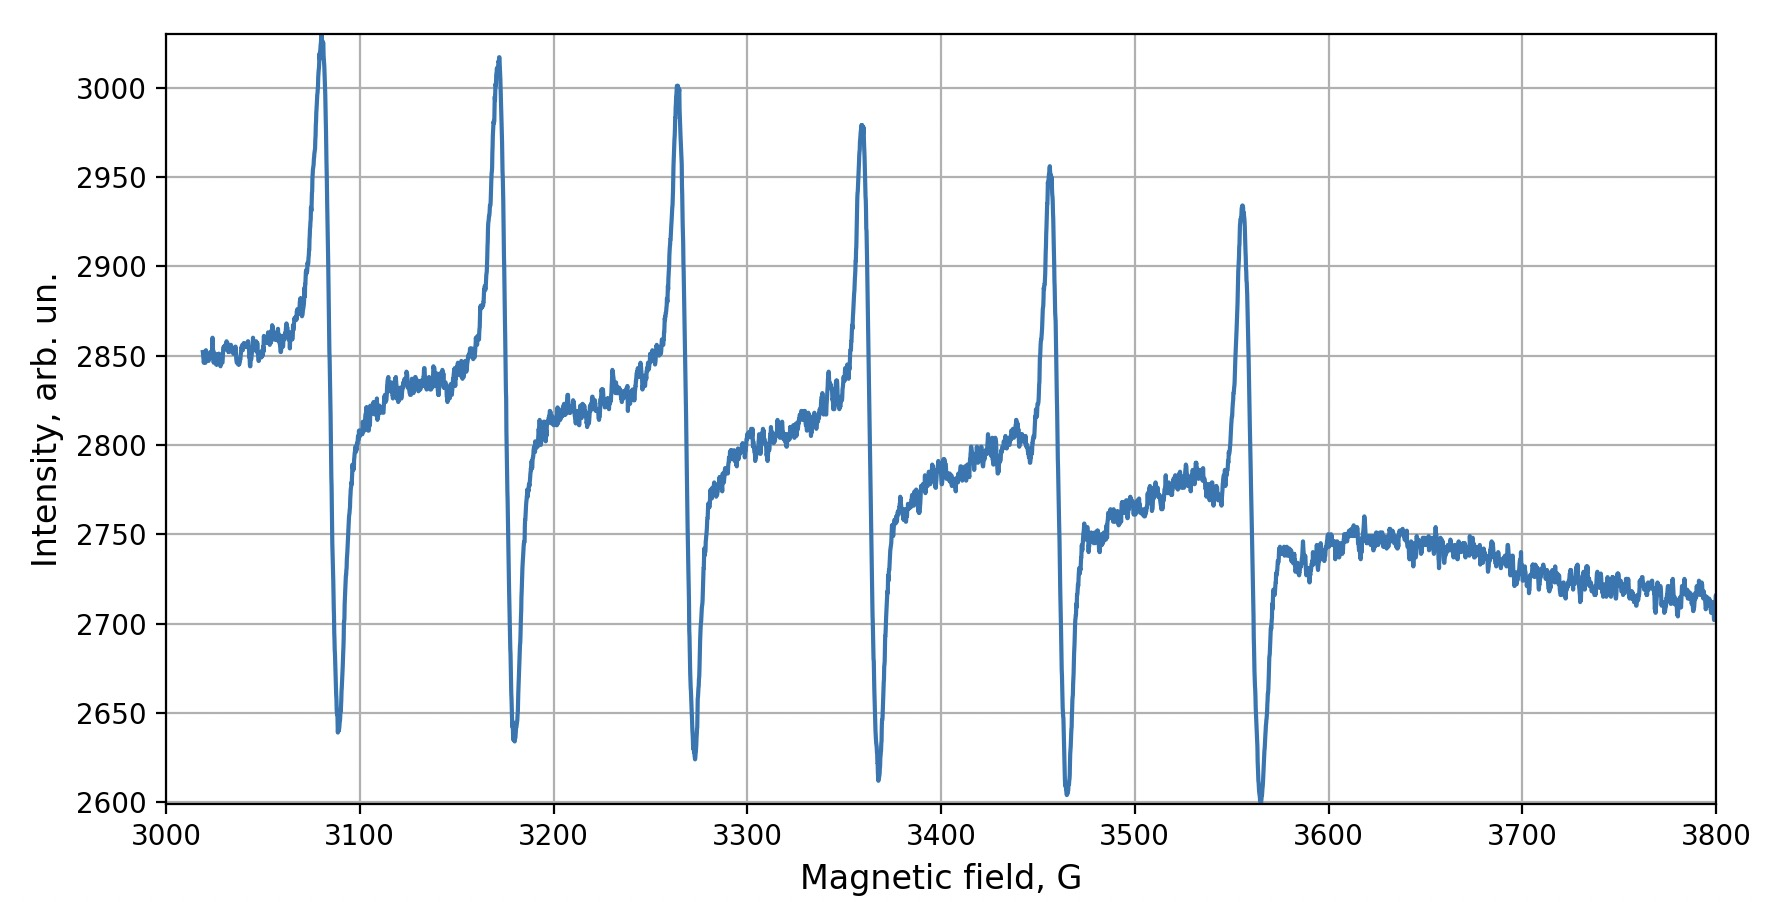
\includegraphics[scale = 0.2]{3.jpeg}
        \caption{Спектр ЭПР порошка $Ca(OH)_2$}
        \label{3}
    \end{figure}

\subsection{Исследование влияния уровня диэлектрических потерь на вид спектров ЭПР}

Были измерены спектры ЭПР для растворов Mn$^{2+}$ низкой концентрации (\hyperref[4]{Рисунок \ref*{4}}) :
\begin{enumerate}
	\item в капилляре;
	\item в пробирке, сохраняя ту же высоту столба жидкости, что и в пункте (a);
	\item в пробирке, сохраняя то же количество парамагнитных центров,
	что и в пункте (a), при таком же объёме, как в пункте (b).
\end{enumerate}
Уровень диэлектрических потерь в исследуемых образцах:

\begin{enumerate}
\item наименьший, сигнал наиболее чёткий.

\item большой. В пробирке должно быть больше парамагнитных цен-
тров, но амплитуда сигнала уменьшается вследствие увеличения
диаметра сосуда с образцом.
\item большой, потому что число парамагнитных центров осталось тем
же, а амплитуда сигнала уменьшилась также из-за увеличения диа-
метра сосуда с образцом.

\end{enumerate}


\begin{figure}[h!]
        \centering
        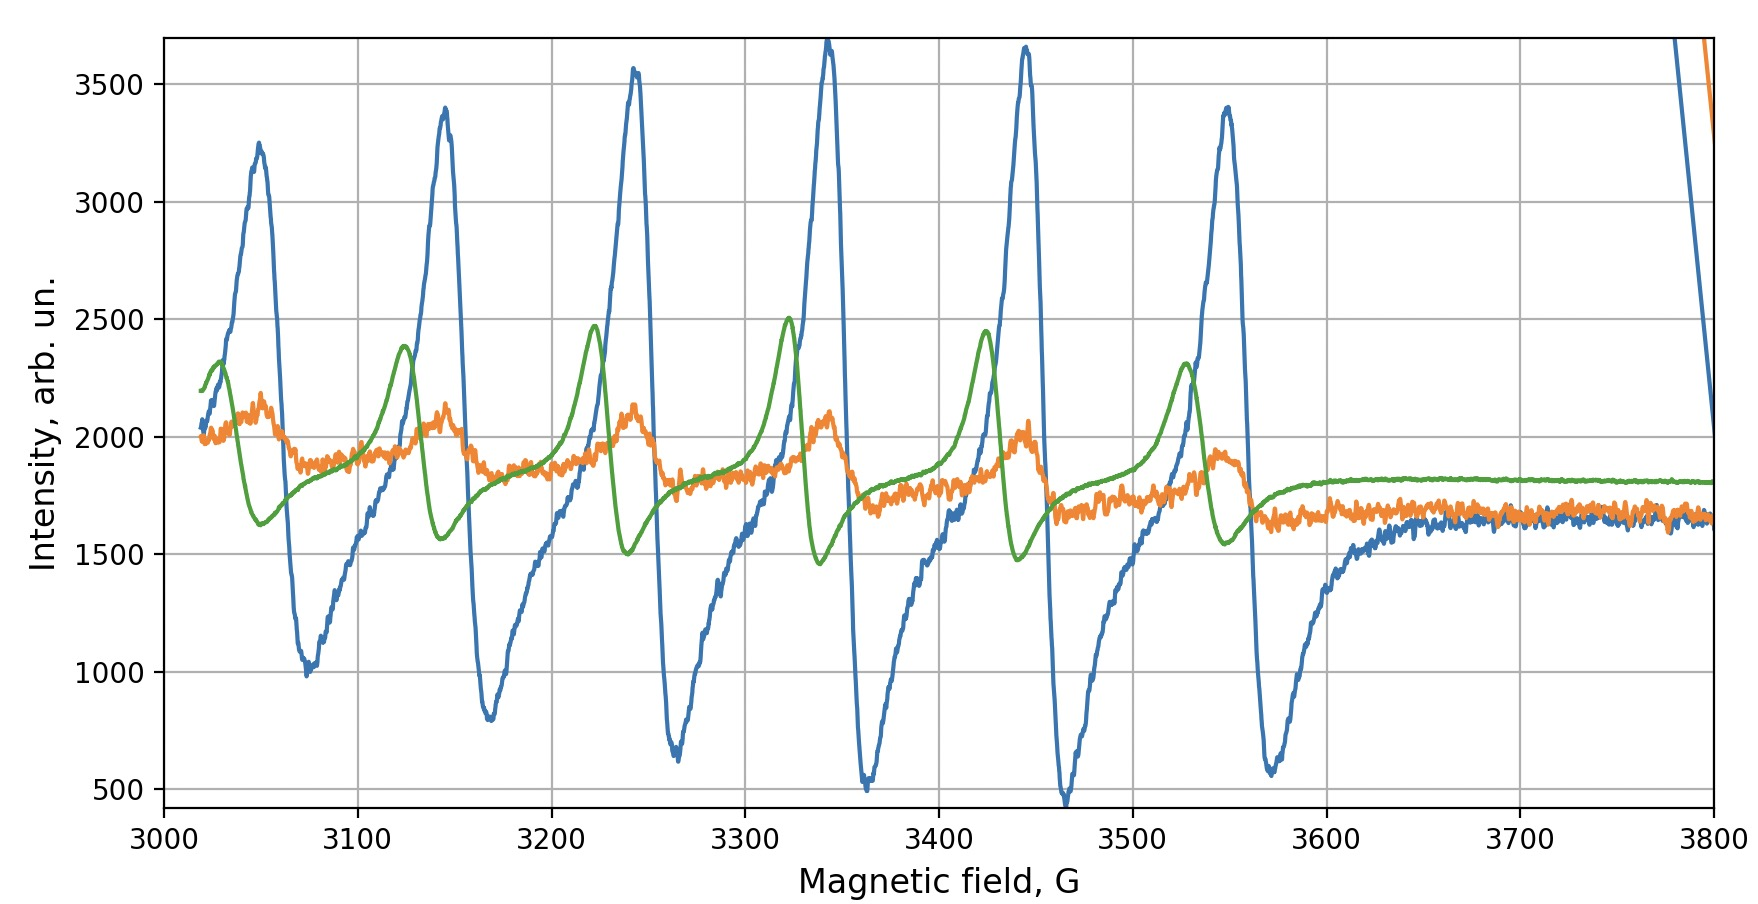
\includegraphics[scale = 0.2]{4.jpeg}
        \caption{Спектр ЭПР соли $Mn^{2+}$ в водном растворе. Синяя кривая - $c = 0.05 M$, капилляр; зеленая кривая - $c = 0.05 M$, пробирка; оранжевая кривая - концентрация парамагнитных центров $c_p = 0.05 M$, пробирка}
        \label{4}
    \end{figure}

    
\subsection{Исследование формы линии}

Исходя из спектров маргнаца при высокой и низкой концентрациях,
можно сделать вывод, что при малых концентрациях спектр лучше опи-
сывается лоренцовой формой кривой, а при повышении концентрации
форма спектра приближается к гауссовой. Реальные линии ЭПР, как
видно, имеют промежуточную форму. Также видно, что спектры ЭПР
исследуемого раствора имеют форму, более близкую к лоренцевой, в се-
редине и более близкую к гауссовой по краям.

\newpage
\section{Выводы}
\begin{enumerate}
    \item На основании зависимости ширины пика от амплитуды высокочастотной модуляции была оценена максимальная амплитуда модуляции постоянного магнитного поля:
    \begin{equation*}
        \delta H_{max} = 1,55 \pm 0,07 \hspace{5pt} \text{Э}.
    \end{equation*}
    
    \item Из зависимости ширины линии поглощения от концентрации марганца была оценена константа спин-спинового взаимодействия и частота столкновений парамагнитных частиц в растворе для $c = 0.6 M$:
    \begin{equation*}
        K_e = (1,3  \pm 0,7) \cdot 10^8 \hspace{5pt} c^{-1}M^{-1}
    \end{equation*}
    \begin{equation*}
         1/\tau_e = 0.08 \pm 0.04 \hspace{5pt} \text{ГГц}
    \end{equation*}
    \item  Была построена зависимости поглощенной энергии СВЧ-поля от концентрации ионов марганца, из которой можно сделать вывод, что при увеличении парамагнитных частиц в растворе увеличивается поглощение энергии. 
    
    \item Из сравнения графиков ЭПР-спектра для марганца в растворе и в кристаллическом виде можно заключить, что спиновый обмен происходит быстрее в веществе в растворенном виде.
    
    \item Используя свойство эквидистантности линий ЭПР, была получена константа сверхтонкого взаимодействия для марганца $a = 101.0 \pm 0.9$ Э.
    
    \item Анализируя вид ЭПР спектров при различных схемах проведения опыта, можно заметить, что наибольший сигнал дает опыт, проведенный с использованием капилляра. Это подтверждает гипотезу о том, что уменьшение объема образца приводит к уменьшению диэлектрических потерь.
    
    \item Исходя из спектров, можно сделать вывод, что спектр лучше описывается лоренцовой формой кривой, но это приближение неидеально. Реальные линии ЭПР, как видно, имеют промежуточную форму, причем при увеличении концентрации спектр стремится к гауссовой форме.
\end{enumerate}

\newpage
\section*{Приложение} \label{prilosh}

\begin{figure}[h!]
  \centering
  \begin{subfigure}[b]{0.3\linewidth}
    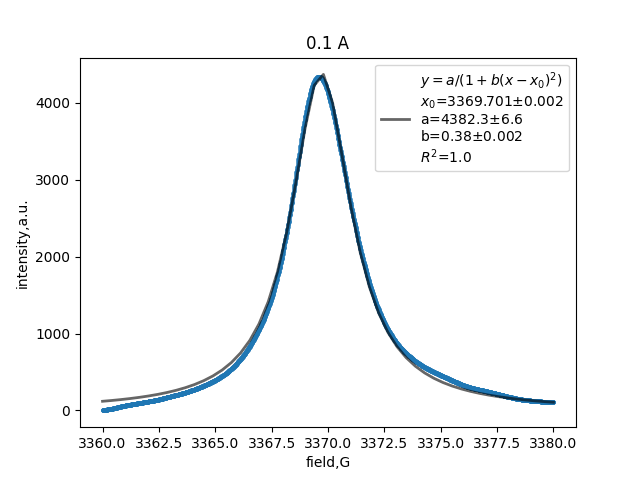
\includegraphics[width=\linewidth]{1/11.png}
    \caption{Ток $I = 0.1$}
  \end{subfigure}
  \begin{subfigure}[b]{0.3\linewidth}
    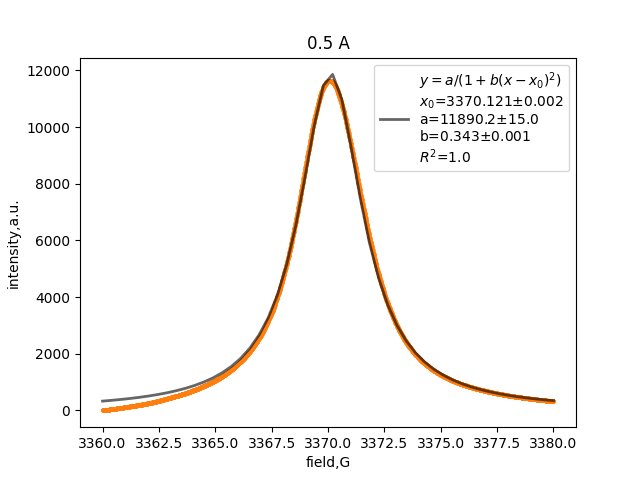
\includegraphics[width=\linewidth]{1/12.png}
    \caption{Ток $I = 0.5$}
  \end{subfigure}
  \begin{subfigure}[b]{0.3\linewidth}
    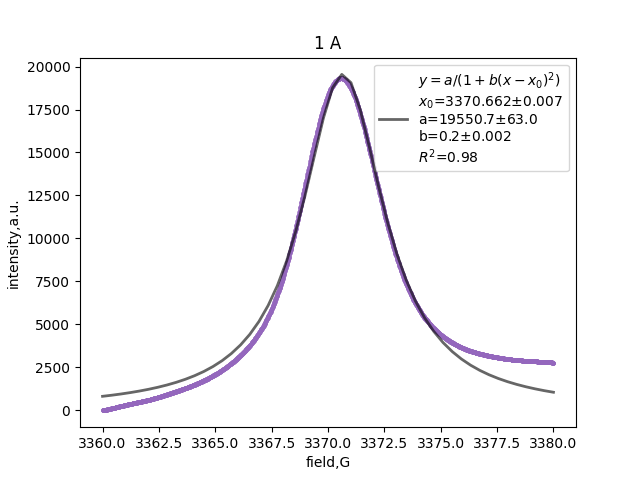
\includegraphics[width=\linewidth]{1/14.png}
    \caption{Ток $I = 1.0$}
  \end{subfigure}
  
  \begin{subfigure}[b]{0.3\linewidth}
    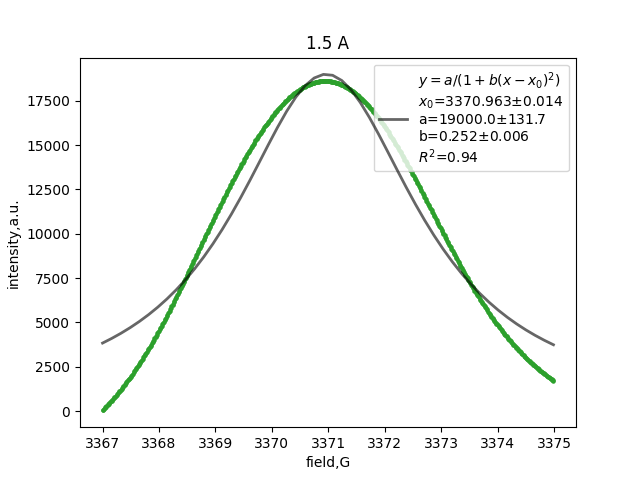
\includegraphics[width=\linewidth]{1/13.png}
    \caption{Ток $I = 1.5$}
  \end{subfigure}
  \begin{subfigure}[b]{0.3\linewidth}
    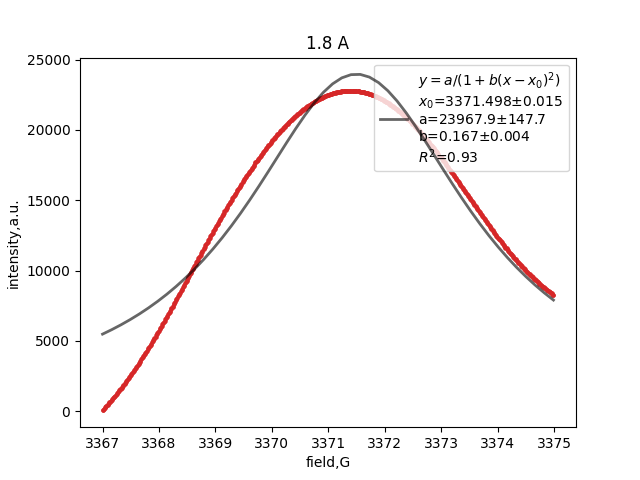
\includegraphics[width=\linewidth]{1/15.png}
    \caption{Ток $I = 1.8$}
  \end{subfigure}
  \caption{Фитирование интегральных интенсивностей спектра ДФПГ ло-
ренцевым контуром}
\label{1__}
\end{figure}



\begin{figure}[h!]
  \centering
  \begin{subfigure}[b]{0.3\linewidth}
    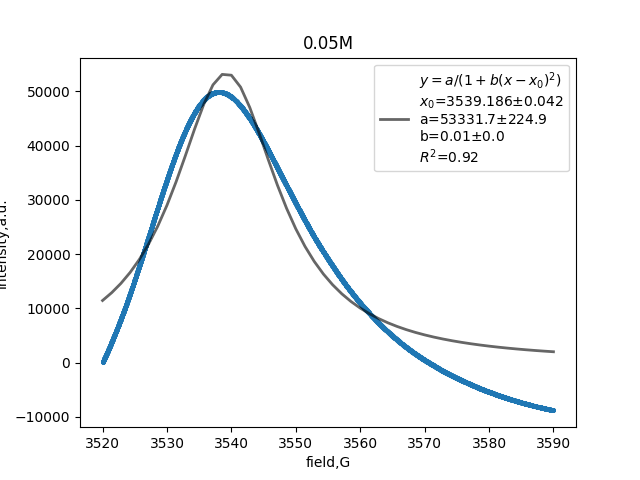
\includegraphics[width=\linewidth]{2.1/21.png}
    \caption{Ток $I = 0.1$}
  \end{subfigure}
  \begin{subfigure}[b]{0.3\linewidth}
    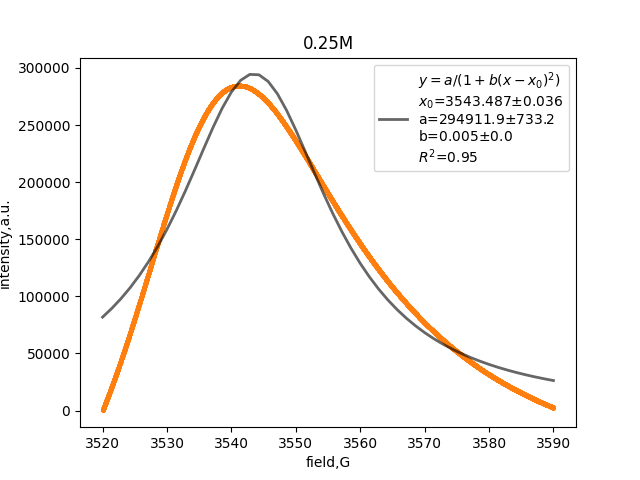
\includegraphics[width=\linewidth]{2.1/22.png}
    \caption{Ток $I = 0.5$}
  \end{subfigure}
  \begin{subfigure}[b]{0.3\linewidth}
    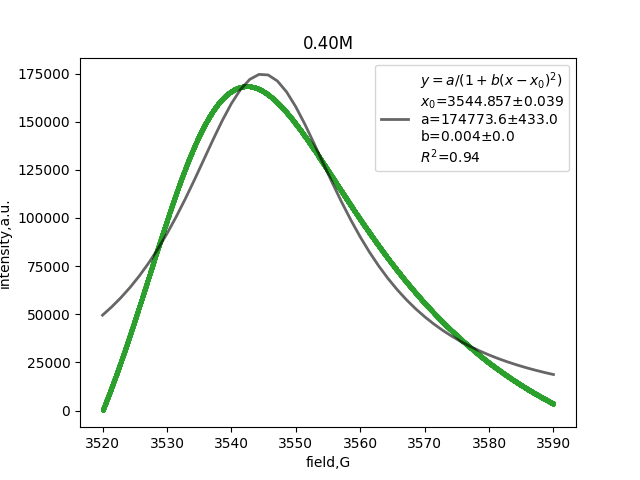
\includegraphics[width=\linewidth]{2.1/23.png}
    \caption{Ток $I = 1.0$}
  \end{subfigure}
  
  \begin{subfigure}[b]{0.3\linewidth}
    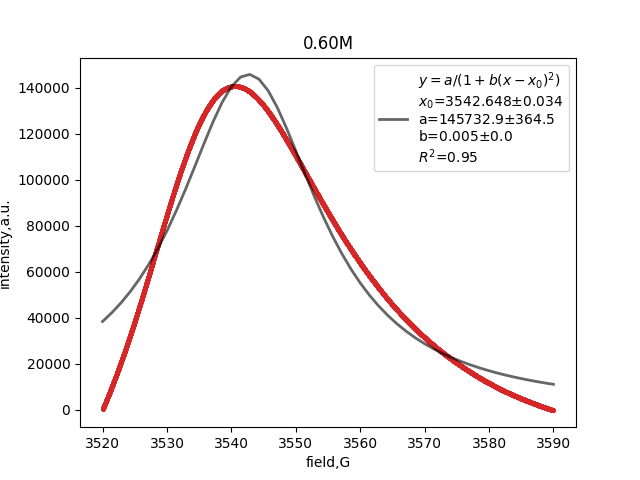
\includegraphics[width=\linewidth]{2.1/24.png}
    \caption{Ток $I = 1.5$}
  \end{subfigure}
  \begin{subfigure}[b]{0.3\linewidth}
    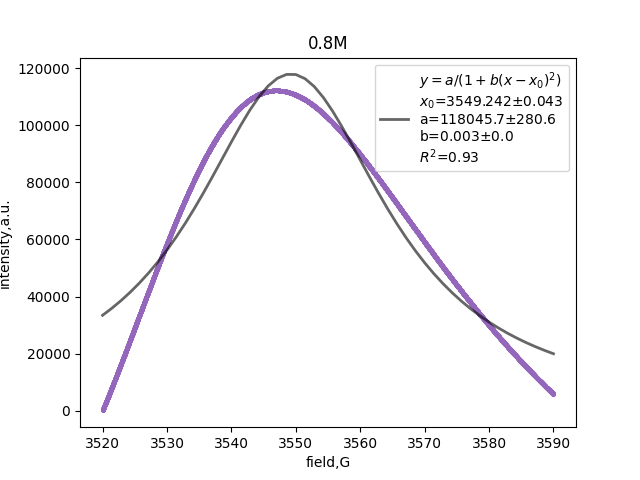
\includegraphics[width=\linewidth]{2.1/25.png}
    \caption{Ток $I = 1.8$}
  \end{subfigure}

  \caption{Фитирование интегральных интенсивностей спектра $MnSO_4$ лоренцевым контуром}
  \label{2__}
\end{figure}





\addcontentsline{toc}{section}{Список используемой литературы}
\begin{thebibliography}{}
    \bibitem{1}  Департамент молекулярной и биологической физики -  "Спектроскопия электронного парамагнитного резонанса"
\end{thebibliography}








\end{document}



